% Options for packages loaded elsewhere
\PassOptionsToPackage{unicode}{hyperref}
\PassOptionsToPackage{hyphens}{url}
\PassOptionsToPackage{dvipsnames,svgnames*,x11names*}{xcolor}
%
\documentclass[
  11pt,
  UTF8]{ctexart}
\usepackage{amsmath,amssymb}
\usepackage{lmodern}
\usepackage{iftex}
\ifPDFTeX
  \usepackage[T1]{fontenc}
  \usepackage[utf8]{inputenc}
  \usepackage{textcomp} % provide euro and other symbols
\else % if luatex or xetex
  \usepackage{unicode-math}
  \defaultfontfeatures{Scale=MatchLowercase}
  \defaultfontfeatures[\rmfamily]{Ligatures=TeX,Scale=1}
\fi
% Use upquote if available, for straight quotes in verbatim environments
\IfFileExists{upquote.sty}{\usepackage{upquote}}{}
\IfFileExists{microtype.sty}{% use microtype if available
  \usepackage[]{microtype}
  \UseMicrotypeSet[protrusion]{basicmath} % disable protrusion for tt fonts
}{}
\makeatletter
\@ifundefined{KOMAClassName}{% if non-KOMA class
  \IfFileExists{parskip.sty}{%
    \usepackage{parskip}
  }{% else
    \setlength{\parindent}{0pt}
    \setlength{\parskip}{6pt plus 2pt minus 1pt}}
}{% if KOMA class
  \KOMAoptions{parskip=half}}
\makeatother
\usepackage{xcolor}
\IfFileExists{xurl.sty}{\usepackage{xurl}}{} % add URL line breaks if available
\IfFileExists{bookmark.sty}{\usepackage{bookmark}}{\usepackage{hyperref}}
\hypersetup{
  pdftitle={2024 年 A 题论文初稿},
  colorlinks=true,
  linkcolor={black},
  filecolor={Maroon},
  citecolor={Blue},
  urlcolor={blue},
  pdfcreator={LaTeX via pandoc}}
\urlstyle{same} % disable monospaced font for URLs
\usepackage[a4paper,margin=2.2cm]{geometry}
\usepackage{longtable,booktabs,array}
\usepackage{graphicx}
\usepackage{float}
\usepackage{calc} % for calculating minipage widths
% Correct order of tables after \paragraph or \subparagraph
\usepackage{etoolbox}
\makeatletter
\patchcmd\longtable{\par}{\if@noskipsec\mbox{}\fi\par}{}{}
\makeatother
% Allow footnotes in longtable head/foot
\IfFileExists{footnotehyper.sty}{\usepackage{footnotehyper}}{\usepackage{footnote}}
\makesavenoteenv{longtable}
\setlength{\emergencystretch}{3em} % prevent overfull lines
\providecommand{\tightlist}{%
  \setlength{\itemsep}{0pt}\setlength{\parskip}{0pt}}
\setcounter{secnumdepth}{5}
\ifLuaTeX
  \usepackage{selnolig}  % disable illegal ligatures
\fi

\title{2024 年 A 题论文初稿}
\author{}
\date{}

\begin{document}
\maketitle

\hypertarget{ux95eeux9898ux5206ux6790}{%
\section{问题分析}\label{ux95eeux9898ux5206ux6790}}

\subsection{问题一分析}

第一问要求确定板凳龙沿给定等距螺线盘入时，各把手中心在
\(0\sim300\,\mathrm{s}\)
内的位置与速度。其本质是受路径约束的多刚体串联系统运动学问题。龙头前把手的运动已知，其余把手的位置由``均位于同一条螺线''和``相邻把手中心距保持不变''共同决定，速度则由刚性距离约束对时间求导得到。

\subsection{问题二分析}

第二问要求确定板凳龙盘入过程中首次发生碰撞的时刻及此时各把手的位置与速度。由于
板凳具有一定宽度，需在第一问定长链运动模型的基础上，将每节板凳表示为由两个把手
中心及板宽确定的矩形，并以非相邻板凳首次接触作为终止条件；同时利用普通龙身尺寸
相同所产生的构型平移性质缩小候选碰撞范围，而长度不同的龙头板凳需单独考察。

\hypertarget{ux6a21ux578bux5047ux8bbe}{%
\section{模型假设}\label{ux6a21ux578bux5047ux8bbe}}

\begin{enumerate}
\def\labelenumi{\arabic{enumi}.}
\tightlist
\item
  将每节板凳视为长度、宽度固定且不发生弹性形变的刚体，把手连接处视为理想铰接，忽略孔径与连接间隙对把手中心位置的影响。
\item
  各把手中心严格位于题目指定的中心轨迹上；相邻把手中心的直线距离在运动过程中保持不变。
\item
  舞龙运动连续、平稳，不发生脱节、跳跃或瞬时速度突变；在分段轨迹连接处满足位置连续与切向连续。
\item
  以地面为二维平面，忽略板凳厚度、把手高度差以及人员运动对几何关系的影响。
\end{enumerate}

\hypertarget{ux7b26ux53f7ux8bf4ux660e}{%
\section{符号说明}\label{ux7b26ux53f7ux8bf4ux660e}}

\begin{longtable}[]{@{}lll@{}}
\toprule
符号 & 含义 & 单位 \\
\midrule
\endhead
\(p\) & 阿基米德螺线螺距 & m \\
\(a\) & 螺线系数，\(a=p/(2\pi)\) & m/rad \\
\(\theta_i(t)\) & \(t\) 时刻第 \(i\) 个把手中心的极角 & rad \\
\(\boldsymbol P_i(t)\) & 第 \(i\) 个把手中心的位置向量 & m \\
\(\boldsymbol T_i(t)\) & 第 \(i\) 个把手沿运动方向的单位切向量 & -- \\
\(v_i(t)\) & 第 \(i\) 个把手的速率 & m/s \\
\(\kappa_i(t)\) & 第 \(i\) 个把手相对于龙头的速度传递系数 & -- \\
\(\boldsymbol V_i(t)\) & 第 \(i\) 个把手的速度向量 & m/s \\
\(L_i\) & 第 \(i-1\) 与第 \(i\) 个把手的中心距 & m \\
\(N\) & 把手中心总数，\(N=224\) & 个 \\
\(\Phi(\theta)\) & \(\int\sqrt{1+\theta^2}\,\mathrm d\theta\) 的原函数 &
-- \\
\(l\) & 普通龙身前、后把手的中心距，\(l=1.65\) & m \\
\(F\) & 普通龙身相邻把手极角之间的递推映射 & -- \\
\(B_i(t)\) & \(t\) 时刻第 \(i\) 节普通龙身所占的闭矩形区域 & -- \\
\(\boldsymbol d_i\) &
相邻把手连杆向量，\(\boldsymbol P_i-\boldsymbol P_{i-1}\) & m \\
\bottomrule
\end{longtable}

\hypertarget{ux6a21ux578bux51c6ux5907ux8defux5f84ux7ea6ux675fux5b9aux957fux94feux901aux7528ux6a21ux578b}{%
\section{板凳龙通用运动学模型}\label{ux6a21ux578bux51c6ux5907ux8defux5f84ux7ea6ux675fux5b9aux957fux94feux901aux7528ux6a21ux578b}}

\subsection{板凳龙的几何抽象}

本文将龙头前把手编号为 \(P_0\)，沿龙身方向依次编号至龙尾后把手
\(P_{223}\)。根据板凳长度及孔中心至板头的距离，龙头前、后把手的中心距为 \[
L_1=3.41-2\times0.275=2.86\ \mathrm m,
\] 其余相邻把手的中心距均为 \[
L_i=2.20-2\times0.275=1.65\ \mathrm m,\qquad i=2,\ldots,223.
\]

\subsection{路径约束与位置递推}\label{sec:general-position}

设所有把手依次位于一条参数曲线 \(\boldsymbol r(u)\) 上，即 \[
\boldsymbol P_i(t)=\boldsymbol r\!\left(u_i(t)\right),\qquad i=0,1,\ldots,N-1.
\] 龙头参数 \(u_0(t)\) 由其弧长运动规律确定。其余把手满足定长约束 \[
G_i(u_{i-1},u_i)
=\left\|\boldsymbol r(u_i)-\boldsymbol r(u_{i-1})\right\|^2-L_i^2=0.
\] 给定 \(u_{i-1}\) 后，在龙身延伸方向选取最近的可行根，即可依次得到
\(u_i\)。这构成全文的位置递推模型。由于五个问题仅在中心路径及附加约束上有所不同，
后续只需给定相应的路径方程、运动方向和参数范围，即可复用上述定长链模型，而不依赖
路径是螺线、圆弧还是分段复合曲线。

\subsection{刚性约束下的速度传递}\label{sec:general-velocity}

令 \(\boldsymbol T_i\) 为轨迹运动方向的单位切向量，且
\(\boldsymbol V_i=v_i\boldsymbol T_i\)。对
\(\|\boldsymbol d_i\|^2=L_i^2\) 关于时间求导，有 \[
\boldsymbol d_i^{\mathsf T}(\boldsymbol V_i-\boldsymbol V_{i-1})=0.
\] 于是得到通用速度递推式 \[
v_i=v_{i-1}
\frac{\boldsymbol d_i^{\mathsf T}\boldsymbol T_{i-1}}
{\boldsymbol d_i^{\mathsf T}\boldsymbol T_i},
\qquad i=1,2,\ldots,N-1.
\] 当轨迹几何和各把手位置确定后，定义速度传递系数
\[
\kappa_i=\prod_{j=1}^{i}
\frac{\boldsymbol d_j^{\mathsf T}\boldsymbol T_{j-1}}
{\boldsymbol d_j^{\mathsf T}\boldsymbol T_j},
\]
\begin{figure}[H]
\centering
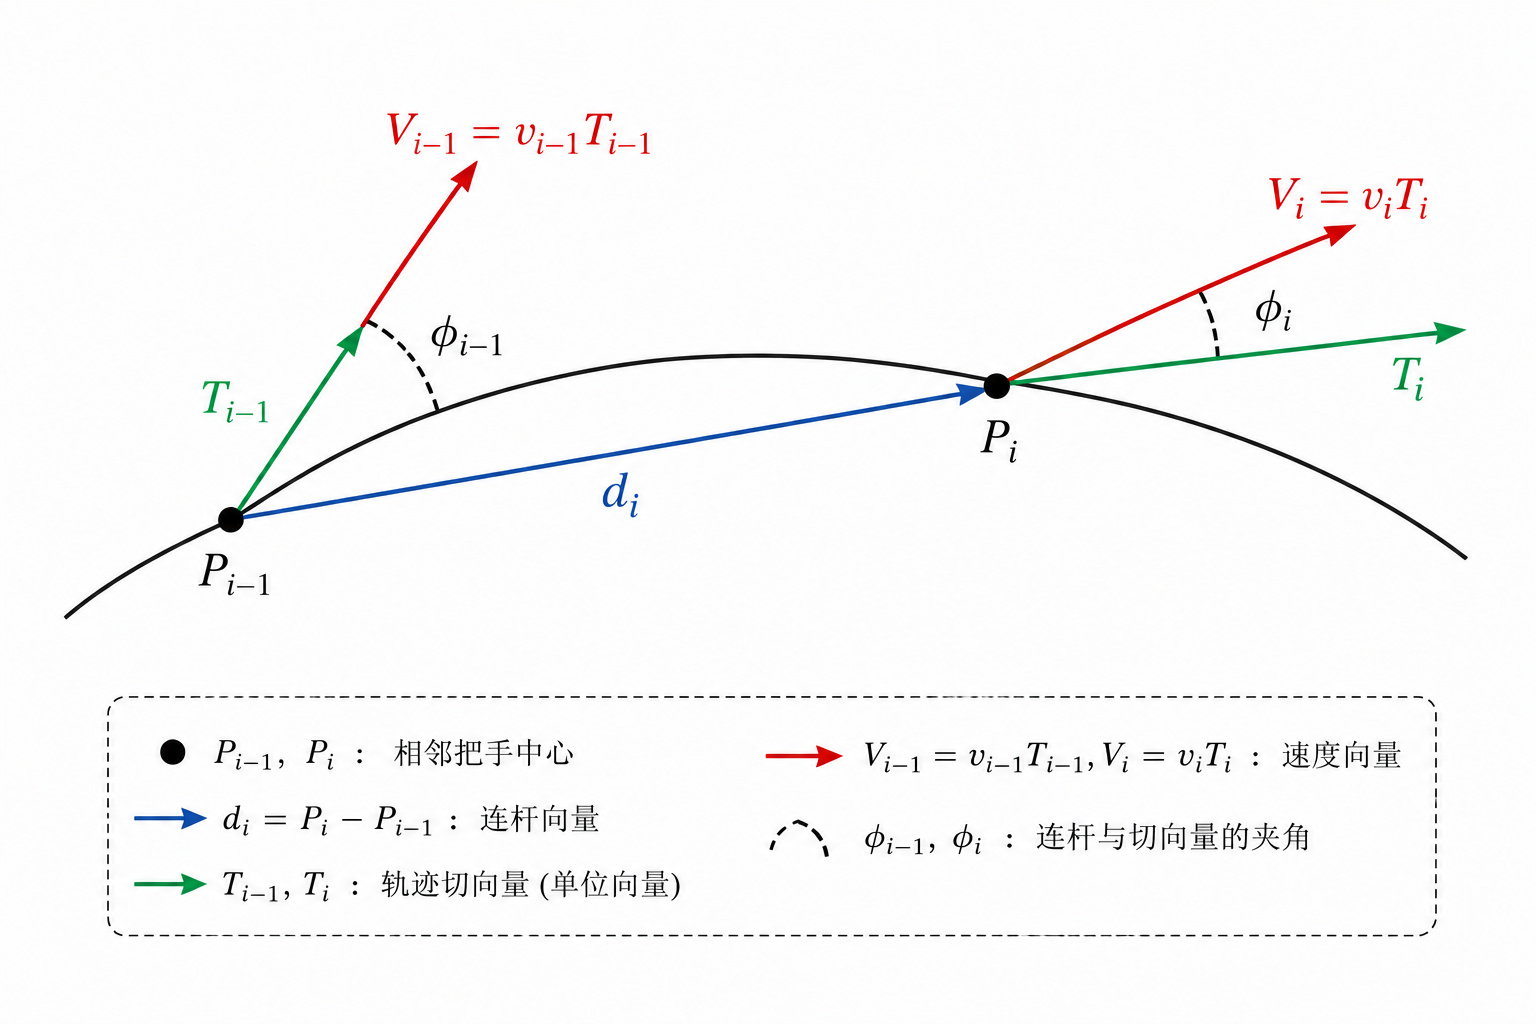
\includegraphics[width=0.82\textwidth]{../figures/velocity_transfer.jpg}
\caption{相邻把手之间的速度传递几何关系}
\label{fig:velocity-transfer}
\end{figure}

则 \(v_i=\kappa_i v_0\)。因此各把手速度均与龙头速度成正比，该性质将在问题五的
最大龙头速度求解中直接使用。

\hypertarget{ux95eeux9898ux4e00ux6a21ux578bux7684ux5efaux7acbux4e0eux6c42ux89e3}{%
\section{问题一模型的建立与求解}\label{ux95eeux9898ux4e00ux6a21ux578bux7684ux5efaux7acbux4e0eux6c42ux89e3}}

\hypertarget{ux963fux57faux7c73ux5fb7ux87baux7ebfux53c2ux6570ux5316}{%
\subsection{阿基米德螺线与初始条件}\label{ux963fux57faux7c73ux5fb7ux87baux7ebfux53c2ux6570ux5316}}

等距螺线的极坐标方程为 \[
r=a\theta,\qquad a=\frac{p}{2\pi}=\frac{0.55}{2\pi}.
\] 取螺线中心为原点、初始点 \(A\) 所在射线为 \(x\)
轴正方向，则把手位置可写为 \[
\boldsymbol P(\theta)
=a\theta(\cos\theta,\sin\theta)^{\mathsf T}.
\] 初始时龙头位于第 16 圈，故 \(\theta_0(0)=32\pi\)，且
\(\boldsymbol P_0(0)=(8.8,0)^{\mathsf T}\,\mathrm m\)。顺时针向内盘入对应
\(\theta\) 随时间减小。

\hypertarget{ux9f99ux5934ux524dux628aux624bux7684ux5f27ux957fux65b9ux7a0b}{%
\subsection{龙头前把手的弧长方程}\label{ux9f99ux5934ux524dux628aux624bux7684ux5f27ux957fux65b9ux7a0b}}

螺线参数导数的模为 \[
\left\|\frac{\mathrm d\boldsymbol P}{\mathrm d\theta}\right\|
=a\sqrt{1+\theta^2}.
\] 定义 \[
\Phi(\theta)=\frac12\left[\theta\sqrt{1+\theta^2}
+\operatorname{arsinh}(\theta)\right].
\] 由于龙头前把手以 \(1\,\mathrm{m/s}\) 匀速运动，\(t\) 秒内走过的弧长为
\(t\)，从而 \[
a\left[\Phi(32\pi)-\Phi\bigl(\theta_0(t)\bigr)\right]=t.
\] 该方程左端关于 \(\theta_0\) 单调，因此在 \([0,32\pi]\)
内具有唯一解。

\hypertarget{ux5176ux4f59ux628aux624bux7684ux4f4dux7f6eux9012ux63a8}{%
\subsection{位置递推方程的具体化}\label{ux5176ux4f59ux628aux624bux7684ux4f4dux7f6eux9012ux63a8}}

记 \(\Delta_i=\theta_i-\theta_{i-1}>0\)。由相邻把手的欧氏距离约束得 \[
a^2\!\left[\theta_i^2+\theta_{i-1}^2
-2\theta_i\theta_{i-1}\cos(\theta_i-\theta_{i-1})\right]=L_i^2.
\] 按照第~\ref{sec:general-position}节的通用位置递推模型，对每个 \(i\) 取满足
\(\theta_i>\theta_{i-1}\) 的最近根，依次得到 \[
\theta_0<\theta_1<\cdots<\theta_{223}.
\] 随后代入螺线参数方程即可得到全部把手的直角坐标。

\hypertarget{ux901fux5ea6ux9012ux63a8}{%
\subsection{螺线切向量与速度求解}\label{ux901fux5ea6ux9012ux63a8}}

螺线沿 \(\theta\) 增大方向的导向量为 \[
\boldsymbol P'(\theta)
=a(\cos\theta-\theta\sin\theta,\,
\sin\theta+\theta\cos\theta)^{\mathsf T}.
\] 由于实际盘入方向为 \(\theta\) 减小方向，单位切向量为 \[
\boldsymbol T(\theta)=-\frac{\boldsymbol P'(\theta)}{a\sqrt{1+\theta^2}}.
\] 将其代入第~\ref{sec:general-velocity}节的通用速度传递模型，并令 \(v_0=1\,\mathrm{m/s}\)，
即可逐节得到每一整数秒全部 224 个把手的速度大小。

\hypertarget{ux6570ux503cux6c42ux89e3ux6d41ux7a0b}{%
\subsection{数值求解算法}\label{ux6570ux503cux6c42ux89e3ux6d41ux7a0b}}

对 \(t=0,1,\ldots,300\)，采用如下递推算法计算整条板凳龙的状态：首先利用弧长方程的
单调性，以相邻时刻的极角为区间端点，使用 \textbf{Brent 区间求根法}求得
\(\theta_0(t)\)；随后对 \(i=1,\ldots,223\)，从 \(\theta_{i-1}(t)\) 右侧进行
\textbf{自适应变号扫描}，锁定距离残差的第一个变号区间，再用 Brent 法精化，从而获得
最近正向根 \(\theta_i(t)\)，避免误选多圈螺线上的远处根。最后将极角转换为直角坐标，
并按第~\ref{sec:general-velocity}节的解析速度公式由龙头向龙尾逐节递推速度。计算结果写入
\texttt{result1.xlsx} 并保留 6 位小数；定长、弧长及速度一致性检验用于验证算法结果。

\begin{figure}[H]
\centering
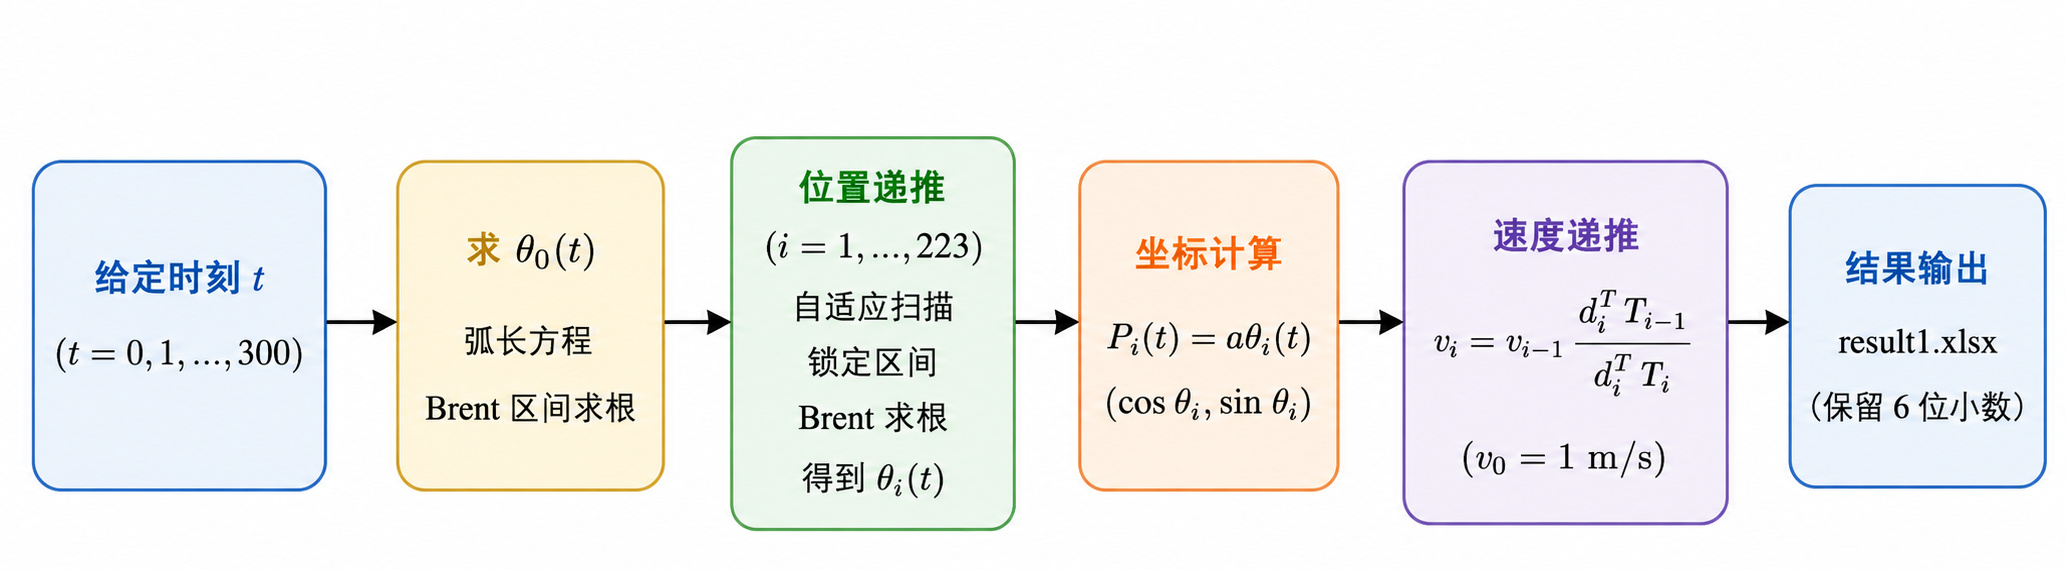
\includegraphics[width=\textwidth]{../figures/q1_numerical_flow.jpg}
\caption{问题一的数值求解流程}
\label{fig:q1-numerical-flow}
\end{figure}

\hypertarget{ux8ba1ux7b97ux7ed3ux679c}{%
\subsection{计算结果}\label{ux8ba1ux7b97ux7ed3ux679c}}

\hypertarget{ux4ee3ux8868ux628aux624bux7684ux4f4dux7f6e}{%
\subsubsection{代表把手的位置}\label{ux4ee3ux8868ux628aux624bux7684ux4f4dux7f6e}}

\begin{longtable}[]{@{}lrrrrrr@{}}
\toprule
把手坐标/m & 0 s & 60 s & 120 s & 180 s & 240 s & 300 s \\
\midrule
\endhead
龙头 (x) & 8.800000 & 5.799209 & -4.084887 & -2.963609 & 2.594494 &
4.420274 \\
龙头 (y) & 0.000000 & -5.771092 & -6.304479 & 6.094780 & -5.356743 &
2.320429 \\
第1节龙身 (x) & 8.363824 & 7.456758 & -1.445473 & -5.237118 & 4.821221 &
2.459489 \\
第1节龙身 (y) & 2.826544 & -3.440399 & -7.405883 & 4.359627 & -3.561949
& 4.402476 \\
第51节龙身 (x) & -9.518732 & -8.686317 & -5.543150 & 2.890455 & 5.980011
& -6.301346 \\
第51节龙身 (y) & 1.341137 & 2.540108 & 6.377946 & 7.249289 & -3.827758 &
0.465829 \\
第101节龙身 (x) & 2.913983 & 5.687116 & 5.361939 & 1.898794 & -4.917371
& -6.237722 \\
第101节龙身 (y) & -9.918311 & -8.001384 & -7.557638 & -8.471614 &
-6.379874 & 3.936008 \\
第151节龙身 (x) & 10.861726 & 6.682311 & 2.388757 & 1.005154 & 2.965378
& 7.040740 \\
第151节龙身 (y) & 1.828753 & 8.134544 & 9.727411 & 9.424751 & 8.399721 &
4.393013 \\
第201节龙身 (x) & 4.555102 & -6.619664 & -10.627211 & -9.287720 &
-7.457151 & -7.458662 \\
第201节龙身 (y) & 10.725118 & 9.025570 & 1.359847 & -4.246673 &
-6.180726 & -5.263384 \\
龙尾（后）(x) & -5.305444 & 7.364557 & 10.974348 & 7.383896 & 3.241051 &
1.785033 \\
龙尾（后）(y) & -10.676584 & -8.797992 & 0.843473 & 7.492370 & 9.469336
& 9.301164 \\
\bottomrule
\end{longtable}

\hypertarget{ux4ee3ux8868ux628aux624bux7684ux901fux5ea6}{%
\subsubsection{代表把手的速度}\label{ux4ee3ux8868ux628aux624bux7684ux901fux5ea6}}

\begin{longtable}[]{@{}lrrrrrr@{}}
\toprule
把手速度/(m/s) & 0 s & 60 s & 120 s & 180 s & 240 s & 300 s \\
\midrule
\endhead
龙头 & 1.000000 & 1.000000 & 1.000000 & 1.000000 & 1.000000 &
1.000000 \\
第1节龙身 & 0.999971 & 0.999961 & 0.999945 & 0.999917 & 0.999859 &
0.999709 \\
第51节龙身 & 0.999742 & 0.999662 & 0.999538 & 0.999331 & 0.998941 &
0.998065 \\
第101节龙身 & 0.999575 & 0.999453 & 0.999269 & 0.998971 & 0.998435 &
0.997302 \\
第151节龙身 & 0.999448 & 0.999299 & 0.999078 & 0.998727 & 0.998115 &
0.996861 \\
第201节龙身 & 0.999348 & 0.999180 & 0.998935 & 0.998551 & 0.997894 &
0.996574 \\
龙尾（后） & 0.999311 & 0.999136 & 0.998883 & 0.998489 & 0.997816 &
0.996478 \\
\bottomrule
\end{longtable}

结果表明，在给定时间范围内，除龙头保持 \(1\,\mathrm{m/s}\)
外，其余把手速度均略低于龙头速度，且总体上沿龙身向后逐渐减小。随着盘入程度加深、局部曲率增大，速度传递系数与
1 的偏差逐渐增大。

\hypertarget{ux7ed3ux679cux9a8cux8bc1ux4e0eux8befux5deeux5206ux6790}{%
\subsection{结果验证与误差分析}\label{ux7ed3ux679cux9a8cux8bc1ux4e0eux8befux5deeux5206ux6790}}

对全部整数时刻进行数值检验，相邻把手定长约束的最大绝对残差为
\(6.461\times10^{-13}\,\mathrm m\)，龙头弧长方程的最大残差为
\(1.990\times10^{-13}\,\mathrm m\)，且始终满足
\(\theta_0<\theta_1<\cdots<\theta_{223}\)，说明首根扫描未发生根分支误选；进一步将刚性杆速度递推
与弦长隐函数微分结果及步长为 \(10^{-3}\,\mathrm s\) 的中心差分结果交叉比较，前两种解析方法的
最大绝对偏差为 \(5.662\times10^{-15}\,\mathrm{m/s}\)，解析速度向量与中心差分的最大相对误差为
\(6.360\times10^{-9}\)。上述误差均远小于结果保留 6 位小数所需精度，验证了位置递推、首根选择和
速度传递模型的正确性。

\section{问题二模型的建立}

\subsection{普通龙身首次碰撞对象的化简}

沿用问题一的螺线参数方程与把手编号。对普通龙身有 \(L_i=l=1.65\,\mathrm m\)。由
第~\ref{sec:general-position}节的定长约束及最近根选取规则，给定其前把手极角
\(\theta_i\) 后，后把手极角由唯一映射 \(F\) 确定：
\[
\theta_{i+1}=F(\theta_i),\qquad
\theta_{i+k}=F^k(\theta_i).
\]
该映射只由螺线参数和普通龙身的把手中心距 \(l\) 决定，与编号 \(i\) 无关。

记 \(B_i(t)\) 为第 \(i\) 节普通龙身在时刻 \(t\) 所占的闭矩形区域，并约定碰撞仅指
无连接关系的板凳发生接触或重叠。下面证明：若首次普通龙身之间的碰撞存在，则其中
必有第 1 节普通龙身。

设时刻 \(t\) 有 \(B_i(t)\cap B_j(t)\ne\varnothing\)，其中 \(j\geq i+2\)。考虑
板凳龙从外向内连续盘入的完整过程。由于 \(\theta_1(t)\) 严格单调减小，且
\(\theta_i(t)>\theta_1(t)\)，存在唯一的较早时刻 \(\tau<t\)，满足
\[
\theta_1(\tau)=\theta_i(t).
\]
对任意 \(k=1,2,\ldots,j-i+1\)，利用同一映射 \(F\) 递推可得
\[
\theta_k(\tau)
=F^{k-1}\!\left(\theta_1(\tau)\right)
=F^{k-1}\!\left(\theta_i(t)\right)
=\theta_{i+k-1}(t).
\]
普通龙身的长度、宽度以及把手相对板端的位置均相同，故一节板凳的闭矩形区域由其
前、后把手位置唯一确定。于是
\[
B_k(\tau)=B_{i+k-1}(t),
\qquad k=1,2,\ldots,j-i+1.
\]
特别地，
\[
B_1(\tau)\cap B_{j-i+1}(\tau)
=B_i(t)\cap B_j(t)\ne\varnothing.
\]
因此，任意一次不涉及第 1 节普通龙身的普通龙身碰撞，都对应于一次发生时间更早且
涉及第 1 节普通龙身的碰撞。若首次碰撞时刻为 \(t^*\)，假设参与碰撞的两节普通
龙身编号均大于 1，便可由上式构造出 \(\tau<t^*\) 的碰撞，与首次性矛盾。故
\[
\boxed{\text{若首次碰撞发生在普通龙身之间，则必然涉及第 1 节普通龙身。}}
\]
龙头板凳的把手中心距为 \(2.86\,\mathrm m\)，不服从普通龙身的映射 \(F\)，因而上述
结论不包含龙头与龙身之间的碰撞。

\end{document}
